\documentclass[11pt]{article}

\usepackage[a4paper, margin=1in]{geometry}
\usepackage{mathtools}
\usepackage{outlines}
\usepackage{amsmath}
\usepackage{pdfpages}
\usepackage{verbatim}
\usepackage{listings}
\usepackage{algorithm}
\usepackage[noend]{algpseudocode}
% \usepackage[dvipsnames]{xcolor}
\usepackage[english]{babel}
\usepackage[labelfont=bf]{caption}
\usepackage{hyperref}
\usepackage{subcaption}
\usepackage{array}
\usepackage{longtable}
%\usepackage[T1]{fontenc}
\usepackage{titlesec, blindtext, color}
\usepackage{float}
\usepackage{graphicx}
\usepackage{xcolor}
\pagecolor{white}
\definecolor{gray75}{gray}{0.75}
\newcommand{\hsp}{\hspace{10pt}}
\titleformat{\section}[hang]{\Huge\bfseries}{\thesection\hsp\textcolor{gray75}{|}\hsp}{0pt}{\Huge\bfseries}

\captionsetup{labelfont=bf}

\makeatletter
\def\BState{\State\hskip-\ALG@thistlm}
\makeatother

\definecolor{codegreen}{rgb}{0,0.6,0}
\definecolor{codegray}{rgb}{0.5,0.5,0.5}
\definecolor{codepurple}{rgb}{0.58,0,0.82}
\definecolor{backcolour}{rgb}{0.95,0.95,0.95}


\lstdefinestyle{mystyle}{
    backgroundcolor=\color{backcolour},   
    commentstyle=\color{codegreen},
    keywordstyle=\color{blue},
    numberstyle=\tiny\color{codegray},
    stringstyle=\color{orange},
    basicstyle=\ttfamily\footnotesize,
    breakatwhitespace=false,         
    breaklines=true,                 
    captionpos=b,                    
    keepspaces=true,                 
    numbers=left,                    
    numbersep=5pt,                  
    showspaces=false,                
    showstringspaces=false,
    showtabs=false,                  
    tabsize=2
}

\lstset{style=mystyle}

\includeonly{
    chapters/introduction,
    chapters/coap,
    chapters/mqtt,
    chapters/collector
}


\begin{document}
\begin{titlepage}
    \begin{center}
        \begin{figure}
            
\includegraphics[width=\textwidth]{img/marchio_unipi_pant541-eps-converted-to.pdf}         
        \end{figure}
        {\Large
        Artificial Intelligence and Data Engineering\\
        \vspace{5mm} %5mm vertical space
        Internet of Things}\\
        \vspace{30mm} %5mm vertical space
        {\Huge\textbf{\textit{IoT Smart Irrigation System}}}\\
        \vspace{10mm} %5mm vertical space
        {\Large Project Documentation}\\
        \par\noindent\rule{\textwidth}{0.4pt}
            \begin{flushright}
                \textit{TEAM MEMBERS}:\\
                Edoardo Fazzari\\ 
                Mirco Ramo\\
        	
            \end{flushright}
            \vfill
        Academic Year: 2020/2021\\        
    \end{center}
\end{titlepage} 
   
\tableofcontents

\section{Introduction}
Agriculture is one of the most fundamental resource of food production and also plays a vital role in keeping the economy running of every nation by contributing to the Gross Domestic Production. But there are several issues related to traditional methods of agriculture such as excessive wastage of water during field irrigation, dependency on non-renewable power source, time, money, human resource etc. Since every activity now a days is becoming smart, it needs to smartly develop agriculture sector for growth of country. Out project aims at developing a Smart Irrigation System using IoT Technology with the objective of automating the total job, providing adequate water required by crop by monitoring the moisture of soil and climate condition in order to prevent the wastage of water resources, resulting in many advantages for farmers. The irrigation at remote location from home will become easy and more comfortable. In addition, it will not only protect farmers from scorching heat and severe cold but also save their time otherwise required by the to-and-from journey to the field.



\subsection{Deployment Structure}
The objective of this project is to adopt a smart irrigation system to water cultivated fields making use of the local water resources, such as aquifers and reservoirs, in the way of using the water resources as more eco-friendly as possible (e.g., without disrupting aquifers). Thus, we can consider two different locations to takes care: the \textbf{field} and the \textbf{water provisioning site},

For what concern the \textit{water provisioning site}, it is composed of sensors which have the mean of monitoring the water level both of the aquifers and reservoirs. In this way, the system and the user can know where to take water (by default the aquifer). Although, a single device for source may be enough, we decided to deploy multiple water level sensors in the same source in order to avoid errors in the monitoring (e.g., in the case of a single device if it is detected that the reservoir is empty, but it is not, the irrigation system will use the water from the aquifer pointlessly).
All water level sensors will make use of \textit{MQTT} as explained in the "MQTT Network" chapter.


The \textit{field site} is more articulated and will exploit multiple types of sensors and a single type of actuator. The actuator needed is the one capable of providing the water to the plants, which we called "tap actuator". This we be used in conjunction with the other sensors presents in the fields that will monitor the environment, specifically there will be temperature sensors, soil moisture sensors and a rain sensor. 
All these sensors and the tap actuator will exploit \textit{CoAP} as explained in the "CoAP Network" chapter.


\begin{figure}[H]
	\begin{subfigure}{\textwidth}
	\centering
		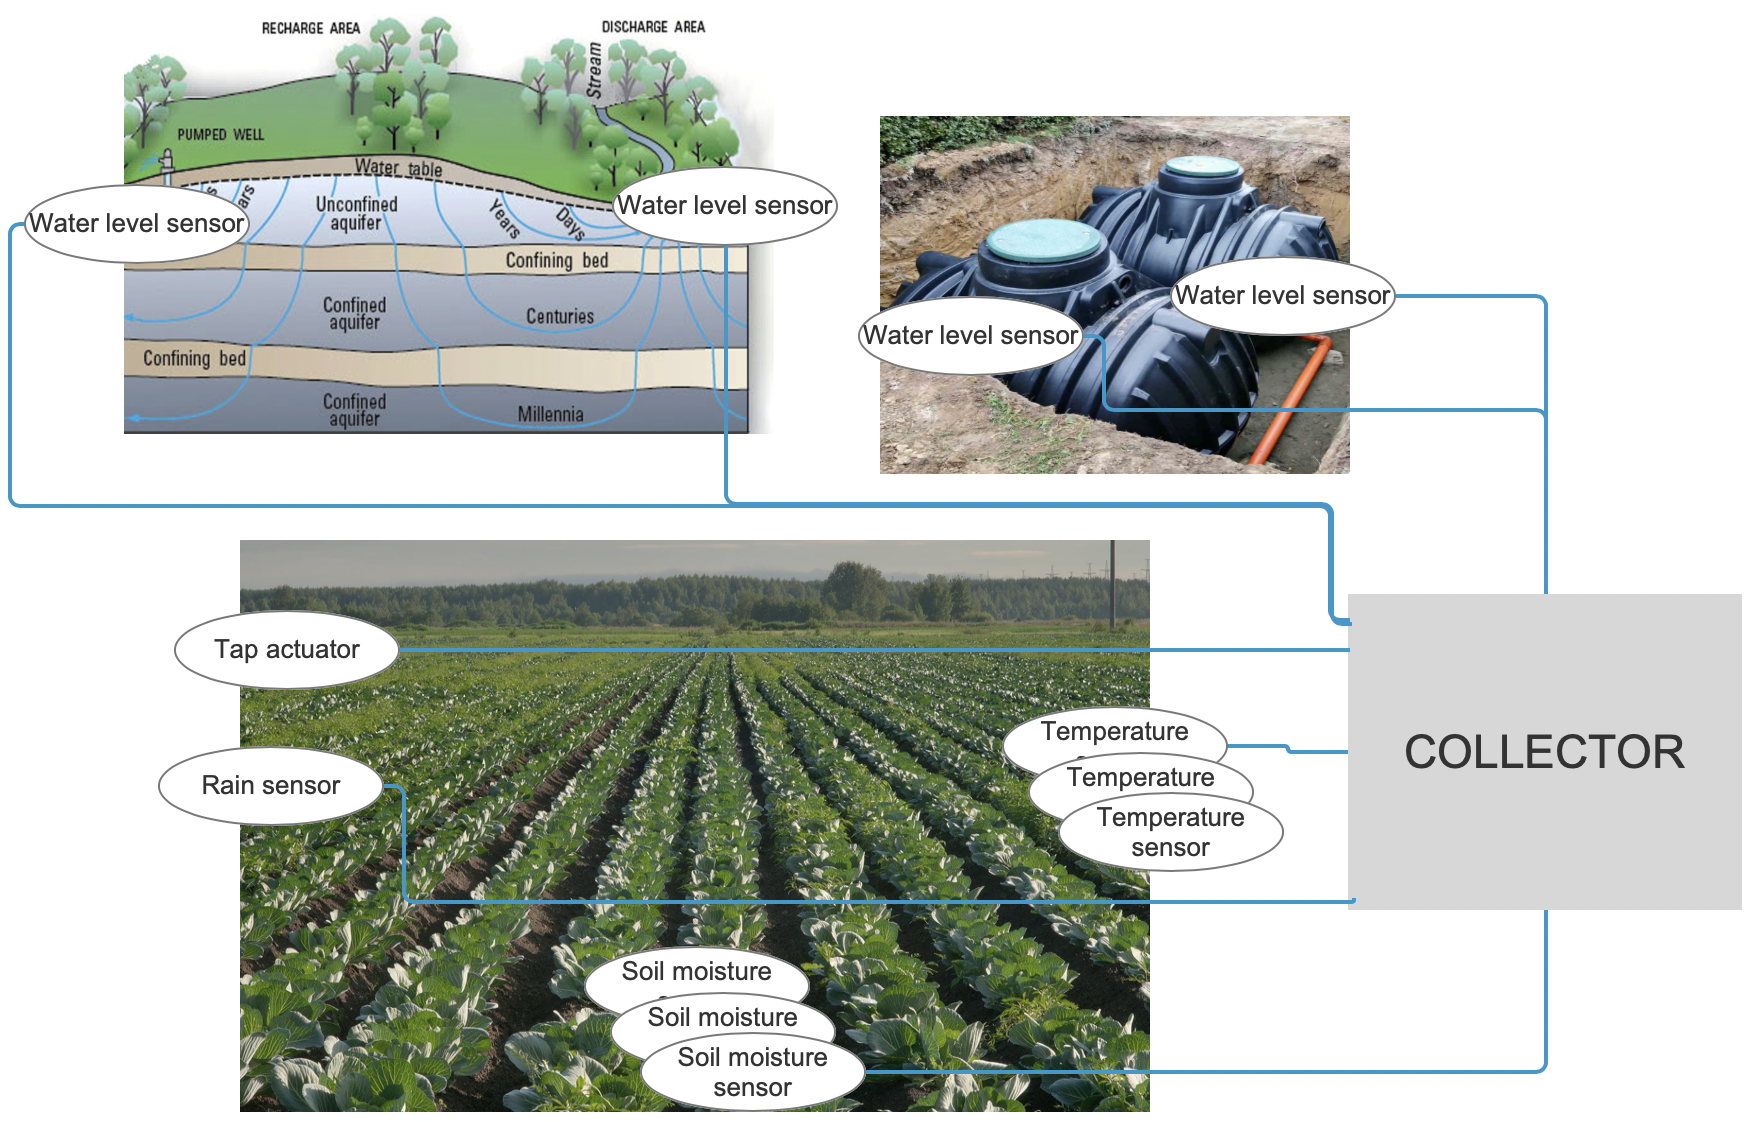
\includegraphics[width=0.66\linewidth]{img/deployment.png} 
	\end{subfigure}
\end{figure}
\section{CoAP Network}
AAa




\subsection{Temperature Sensor}
The temperature sensor measures the local temperature in Celsius (at the Collector level will be given the possibility to display the results in Fahrenheit, see the Collector chapter for further details). The goal of this sensors is to quantify and schedule the water provisioning.

\subsubsection{Resources}
The temperature sensor exposes two resources: the \textit{temperature\_sensor} and the \textit{temperature\_switch} resources.

The \textbf{temperature\_sensor} resource is an observable resource that provides to the clients the temperature acquired by the sensor. The resource not only provides the mere temperature to the clients, but it informs if the temperature is lower or greater than a certain threshold. Hence, the sensor exposes a  \textit{PUT} method, in order to set up the lower or the upper bound for the temperature.

The change of the bounds is done at step, the user will specify the threshold that he/she wants to change through the CLI: upper or lower. At the server side the request will be processed checking if the value arrived is consistent (e.g., the new value for the lower bound is not greater than the upper bound actual value), after those controls the parameter is updated.

The \textbf{temperature\_switch} resource is connected to the \textit{isActive} boolean variable, which indicates if the sensor is operating or not. This is done for turning off the temperature sensor when it is raining in order to save energy, since we do not perform any analysis for irrigating when the weather does that for us. For the reason that we want to change the status of the resources based on the rain sensor, it is implemented a \textit{PUT} method for changing the value of the \textit{isActive} variable.

\subsubsection{Data Generation}
Data is generated every \textit{CLOCK\_SECOND} in order to have a rapid simulation. The value for the temperature is updated using the following algorithm:

\begin{lstlisting}
static void temperature_event_handler(void)
{
    if (!isActive) {
        return; // DOES NOTHING SINCE IT IS TURNED OFF
    }
    
    // extimate new temperature
    srand(time(NULL));
    int new_temp;
    int random = rand() % 4; // generate 0, 1, 2, 3
    
    if (random == 0) // 25% of changing the value
        if (random < 2) // decrease
            new_temp -= VARIATION;
        else // increase
            new_temp += VARIATION;

    // if not equal
    if (new_temp != temperature)
    {
        temperature = new_temp;
        coap_notify_observers(&temperature_sensor);
    }
}
\end{lstlisting}



\subsection{Soil Moisture Sensor}
Soil moisture sensors measure the water content in the soil and can be used to estimate the amount of stored water in the soil horizon. Soil moisture sensors do not measure water in the soil directly. Instead, they measure changes in some other soil property that is related to water content in a predictable way. Checking the different technologies used for measure soil moisture content, we decide to exploit the \textit{soil water potential}\footnote{\textit{Soil water potential} or \textit{soil moisture tension} is a measurement of how tightly water clings to the soil and is expressed in units of pressure called bars. Generally, the drier the soil, the greater the soil water potential and the harder a plant must work to draw water from the soil.}.

\subsubsection{Resources}
The soil moisture sensor exposes two resources: the \textit{soil\_moisture\_sensor} and the \textit{soil\_moisture\_switch} resources.

The \textbf{soil\_moisture\_sensor} resource is an observable resource that provides to the clients the soil moisture tension acquired by the sensor. The resource not only provides the mere tension to the clients, but it informs if the value is lower or greater than a certain threshold. Hence, the sensor exposes a  \textit{PUT} method, in order to set up the lower or the upper bound for the tension\footnote{For the default range value we used the ones indicated here: https://www.metergroup.com/environment/articles/defining-water-potential/ }.

The change of the bounds is done at step, the user will specify the threshold that he/she wants to change through the CLI: upper or lower. At the server side the request will be processed checking if the value arrived is consistent (e.g., the new value for the lower bound is not greater than the upper bound actual value), after those controls the parameter is updated.

The \textbf{soil\_moisture\_switch} resource is connected to the \textit{isActive} boolean variable, which indicates if the sensor is operating or not. This is done for turning off the temperature sensor when it is raining in order to save energy, since we do not perform any analysis for irrigating when the weather does that for us. For the reason that we want to change the status of the resources based on the rain sensor, it is implemented a \textit{PUT} method for changing the value of the \textit{isActive} variable.

\subsubsection{Data Generation}
Data is generated every \textit{CLOCK\_SECOND} in order to have a rapid simulation. The value for the tension is updated using the following algorithm (the same of to the one used for the temperature):

\begin{lstlisting}
static void soil_moisture_event_handler(void)
{
    if (!isActive) {
        return; // DOES NOTHING SINCE IT IS TURNED OFF
    }
    
    // extimate new tension
    srand(time(NULL));
    int new_soilTension = soilTension;
    int random = rand() % 4; // generate 0, 1, 2, 3
    
    if (random == 0) // 25% of changing the value
        if (random < 2) // decrease
            new_soilTension -= VARIATION;
        else // increase
            new_soilTension += VARIATION;

    // if not equal
    if (new_soilTension != soilTension)
    {
        soilTension = new_soilTension;
        coap_notify_observers(&soil_moisture_sensor);
    }
}
\end{lstlisting}



\subsection{Rain Sensor}
Rain sensor or rain switch is a switching device activated by rainfall. It is used for water conservation since it is connected to the automatic irrigation system, which will cause the system to shut down in the event of rainfall in order to do not waste water and to reduce energy consumption.

\subsubsection{Resource}
The only resource provided by the rain sensor is a value indicating if it is raining or not, named \textbf{isRaining} and stored as a boolean. Since we are only interested when the status of the variable change, we opt to use the observable pattern provided by CoAP in order to minimize the number of interactions with the sensor.

The only possible action is the \textbf{GET} method, which will respond with a text saying \textit{"raining"} or \textit{"not raining"} based on the status of \textit{isRaining}.

\subsubsection{Data Generation}
Data is generated every \textit{CLOCK\_SECOND} in order to have a rapid simulation. The value of \textbf{isRaining} flips (i.e., if it was indicating raining it turns to not raining, and vice versa) with a probability of 10\%. This is done in the \textit{rain\_event\_handler} function in the following way:

\begin{lstlisting}
static void rain_event_handler(void)
{
    // check if raining
    srand(time(NULL));
    int random = rand() % 10; // generate 0, 1, ..., 9
    
    bool new_isRaining = isRaining;
    if (random == 0) // 10% of changing the value
        new_isRaining = !isRaining;

    // if not equal, notify
    if (new_isRaining != isRaining) {
        isRaining = new_isRaining;
        coap_notify_observers(&rain_sensor);
    }
}
\end{lstlisting}

In case the value changes, this is notified to all the subscribers.




\subsection{Tap Actuator}
The tap actuator is the device aim at irrigating the fields.

\subsubsection{Resources}
The tap actuator exposes four resources: the \textit{tap\_intensity}, the \textit{tap\_interval}, \textit{tap\_where\_water} and the \textit{tap\_switch}.

The \textbf{tap\_intensity} resource is related to the \textit{intensity} variable, which indicates the volume of water to provide at each simulation. Since we want to pull water form the aquifer or the reservoir, we made this resource observable in the way of better controlling the \textit{water level sensors} in the simulation. The method implemented for this resource are the \textit{GET} and \textit{PUT} methods. The \textit{GET} method respond to the user with a string containing the value of the intensity and, separated by a space, a character value indicating if the water is taken from the aquifer ('A') or the reservoir('R'). On the other hand, the \textit{PUT} method gives to the user the possibility to set up the intensity value updating the current one.

The \textbf{tap\_interval} resource indicates the period of time (expressed in \textit{CLOCK\_SECOND}) between two activations of the tap. This resource can be retrieved using the \textit{GET} method associated to it, and it can be updated using the \textit{PUT} method. The \textit{PUT} method does not only update the value, but it updates also the intensity based on the following formula.

\begin{equation}\label{eq1}
  \begin{gathered}
    \text{intensity} = \text{intensity} * \frac{\text{new\_interval\_value}}{\text{old\_interval\_value}}
  \end{gathered}
\end{equation}

The \textbf{tap\_where\_water} resource is used by the device in order to decide where to takes the water for every irrigation activity. Thus, the resource provide a \textit{PUT} method for changing this value and, for sake of control, we implemented the possibility to retrieve the value through a \textit{GET} method.

The \textbf{tap\_switch} resource works in the same way of the \textbf{temperature\_switch} and \textbf{soil\_moisture\_switch} resources. The meaning of use this type of resource is for not irrigating when raining since it would be a waste.
\section{MQTT Network}

\subsection{Devices}
The MQTT Network will be deployed in the water provisioning site and it is formed by 4 nodes (2 Aquifer Level Detectors and 2 Reservoirs Level Detectors and Actuators). The role of those devices is to monitor the water level in the two sources, in order to always have it enough for the irrigation needs but without the spoil of the natural resources. Each pair of devices communicates the sensed levels  to the Collector, which will compute the mean of the values to more precisely estimate the actual aquifer and reservoir level.


\subsection{Aquifer Level Detector}
The temperature sensor measures the local temperature in Celsius (at the Collector level will be given the possibility to display the results in Fahrenheit, see the Collector chapter for further details). The goal of this sensors is to quantify and schedule the water provisioning.

\subsubsection{Topics}
The temperature sensor exposes two resources: the \textit{temperature\_sensor} and the \textit{temperature\_switch} resources.

The \textbf{temperature\_sensor} resource is an observable resource that provides to the clients the temperature acquired by the sensor. The resource not only provides the mere temperature to the clients, but it informs if the temperature is lower or greater than a certain threshold. Hence, the sensor exposes a  \textit{PUT} method, in order to set up the lower or the upper bound for the temperature.

The change of the bounds is done at step, the user will specify the threshold that he/she wants to change through the CLI: upper or lower. At the server side the request will be processed checking if the value arrived is consistent (e.g., the new value for the lower bound is not greater than the upper bound actual value), after those controls the parameter is updated.

The \textbf{temperature\_switch} resource is connected to the \textit{isActive} boolean variable, which indicates if the sensor is operating or not. This is done for turning off the temperature sensor when it is raining in order to save energy, since we do not perform any analysis for irrigating when the weather does that for us. For the reason that we want to change the status of the resources based on the rain sensor, it is implemented a \textit{PUT} method for changing the value of the \textit{isActive} variable.

\subsubsection{Data Generation}
Data is generated every \textit{CLOCK\_SECOND} in order to have a rapid simulation. The value for the temperature is updated using the following algorithm:

\begin{lstlisting}
static void temperature_event_handler(void)
{
    if (!isActive) {
        return; // DOES NOTHING SINCE IT IS TURNED OFF
    }
    
    // extimate new temperature
    srand(time(NULL));
    int new_temp;
    int random = rand() % 4; // generate 0, 1, 2, 3
    
    if (random == 0) // 25% of changing the value
        if (random < 2) // decrease
            new_temp -= VARIATION;
        else // increase
            new_temp += VARIATION;

    // if not equal
    if (new_temp != temperature)
    {
        temperature = new_temp;
        coap_notify_observers(&temperature_sensor);
    }
}
\end{lstlisting}



\subsection{Reservoir Level Detector and Actuator}
Soil moisture sensors measure the water content in the soil and can be used to estimate the amount of stored water in the soil horizon. Soil moisture sensors do not measure water in the soil directly. Instead, they measure changes in some other soil property that is related to water content in a predictable way. Checking the different technologies used for measure soil moisture content, we decide to exploit the \textit{soil water potential}\footnote{\textit{Soil water potential} or \textit{soil moisture tension} is a measurement of how tightly water clings to the soil and is expressed in units of pressure called bars. Generally, the drier the soil, the greater the soil water potential and the harder a plant must work to draw water from the soil.}.

\subsubsection{Topics}
The soil moisture sensor exposes two resources: the \textit{soil\_moisture\_sensor} and the \textit{soil\_moisture\_switch} resources.

The \textbf{soil\_moisture\_sensor} resource is an observable resource that provides to the clients the soil moisture tension acquired by the sensor. The resource not only provides the mere tension to the clients, but it informs if the value is lower or greater than a certain threshold. Hence, the sensor exposes a  \textit{PUT} method, in order to set up the lower or the upper bound for the tension\footnote{For the default range value we used the ones indicated here: https://www.metergroup.com/environment/articles/defining-water-potential/ }.

The change of the bounds is done at step, the user will specify the threshold that he/she wants to change through the CLI: upper or lower. At the server side the request will be processed checking if the value arrived is consistent (e.g., the new value for the lower bound is not greater than the upper bound actual value), after those controls the parameter is updated.

The \textbf{soil\_moisture\_switch} resource is connected to the \textit{isActive} boolean variable, which indicates if the sensor is operating or not. This is done for turning off the temperature sensor when it is raining in order to save energy, since we do not perform any analysis for irrigating when the weather does that for us. For the reason that we want to change the status of the resources based on the rain sensor, it is implemented a \textit{PUT} method for changing the value of the \textit{isActive} variable.

\subsubsection{Data Generation}
Data is generated every \textit{CLOCK\_SECOND} in order to have a rapid simulation. The value for the tension is updated using the following algorithm (the same of to the one used for the temperature):

\begin{lstlisting}
static void soil_moisture_event_handler(void)
{
    if (!isActive) {
        return; // DOES NOTHING SINCE IT IS TURNED OFF
    }
    
    // extimate new tension
    srand(time(NULL));
    int new_soilTension = soilTension;
    int random = rand() % 4; // generate 0, 1, 2, 3
    
    if (random == 0) // 25% of changing the value
        if (random < 2) // decrease
            new_soilTension -= VARIATION;
        else // increase
            new_soilTension += VARIATION;

    // if not equal
    if (new_soilTension != soilTension)
    {
        soilTension = new_soilTension;
        coap_notify_observers(&soil_moisture_sensor);
    }
}
\end{lstlisting}




\section{Collector}
The \textit{Collector} is the main component of our system. The Collector performs different activities: it collects the data form both MQTT and CoAP sensors; it communicates with the devices in order to perform actions; and it stores all the data collected in \textit{MySQL} in the way they can be visualized through \textbf{Grafana} as indicated in the "Database And Data Visualization" paragraph.

In this chapter, all the subcomponents of the Collector will be explained, which are:  MQTT side, CoAP side, DB connection, Data Visualization, and Automation Irrigation System.

\subsection{Command Line Interface}
The \textit{Collector} exposes a \textbf{Command Line Interface}, through which the user can interact with the system. The commands are printed on the terminal when the application starts and they are the following (otherwise indicated the commands are related to CoAP node):

\begin{itemize}
	\item \textit{getDevicesList}: show list of all available sensors (both CoAP and MQTT).
	\item \textit{getTemp}: get the last temperature registered.
	\item \textit{setTemp $<l/u> <value>$}: set desired temperature for specified bound (l for lower, u for upper). Value is an integer expressed in Celsius/Fahrenheit.
	\item \textit{setUnit $<F/C>$}: change temperature measure unit in C (Celsius) or F (Fahrenheit).
	\item \textit{getWeather}: get if the rain sensor feels rain or not.
	\item \textit{getSoilTension}: get the last soil tension registered.
	\item \textit{setSoilTension $<l/u> <value>$}: set desired tension for specified bound (l for lower, u for upper).
	\item \textit{getTapInterval}: get the interval which the tap operates.
	\item \textit{getTapIntensity}: get the intensity which the tap operates.
	\item \textit{setTapInterval $<seconds>$}: set the interval which the tap operates in seconds (acts also on MQTT nodes).
	\item \textit{setTapIntensity $<value>$}: set the intensity which the tap operates (values is a double).
	\item \textit{getWaterLevels}: print the water levels of aquifer and reservoir (MQTT network related).
	\item \textit{start}: start the automatic irrigation system (Java Thread).
	\item \textit{stop}: stop the automatic irrigation system (Java Thread).
	\item \textit{help}: print the commands list.
	\item \textit{quit}: quit the program.
\end{itemize}




\subsection{MQTT Side}
The Collector works as MQTT client: its role consist on receiving periodic measurements about the water levels and make them available to user commands. It is also in charge of sending commands to the reservoir actuator. This mechanism is implemented through the publish/subscribe model: once the Collector is connected with the MQTT broker (Mosquitto process running on user@iot.dii.unipi.it), it starts publishing commands and receiving the updated measurements.
In order to enhance the modularity, 2 separate classes handle respectively the communication with the aquifer and  with the reservoir, according to topics specified above. Collected measurements are stored into a $<nodeId, value>$ Hashmap, and the actual level is taken as the mean of the 2 levels.

The system can potentially handle any number of MQTT devices.



\subsection{CoAP Side}
The Collector plays the roles of both CoAP client and CoAP server. As far as server functionality is concerned, the Collector has a class (called RegistrationServer, which extends CoapServer) which has the task of allowing CoAP nodes to register for the service. In this way, the Collector can use the registered devices acting as a client in order to obtain the data generated by them and also perform actions as indicated in the "Command Line Interface" paragraph and in the "CoAP Network" chapter.

To ensure greater modularity to the code, it was decided to implement dedicated classes for each device, the implementation details are left out here. What is important to underline, however, is the number of devices that can be registered in the system: we thought that in our environment it is possible to insert one or more temperature sensors, one or more soil sensors, a rain sensor and a single tap actuator. The Collector is able to scale autonomously as the temperature and soil sensors number increase thanks to the use of a \textit{List of CoapClient} objects assigned for each resource exposed by the sensors.


\subsection{Database And Data Visualization}
Since we need to save the data obtained, we have implemented a class called \textit{IrrigationSystemDbManager} dedicated to communicating with MySQL to store the data obtained from the devices every time they change. In fact, each device as indicated in the "CoAP Network" chapter has an observable resource, which generate get requests that are captured by our Collector that will call a dedicated function in the \textit{IrrigationSystemDbManager} class to store the data properly.

The data that are saved in the DB are the following (here the sql code to generate the tables):

\begin{verbatim}
CREATE TABLE IF NOT EXISTS `iot_irrigation_system`.`rain` (
  `idrain` INT NOT NULL AUTO_INCREMENT,
  `timestamp` TIMESTAMP NOT NULL DEFAULT CURRENT_TIMESTAMP,
  `isRaining` TINYINT NOT NULL,
  PRIMARY KEY (`idrain`))
ENGINE = InnoDB;


CREATE TABLE IF NOT EXISTS `iot_irrigation_system`.`soilMoisture` (
  `idsoilMoisture` INT NOT NULL AUTO_INCREMENT,
  `timestamp` TIMESTAMP NOT NULL DEFAULT CURRENT_TIMESTAMP,
  `soilValue` DOUBLE NOT NULL,
  PRIMARY KEY (`idsoilMoisture`))
ENGINE = InnoDB;


CREATE TABLE IF NOT EXISTS `iot_irrigation_system`.`tap` (
  `idtap` INT NOT NULL AUTO_INCREMENT,
  `timestamp` TIMESTAMP NOT NULL DEFAULT CURRENT_TIMESTAMP,
  `intensity` DOUBLE NOT NULL,
  `interval` INT NOT NULL,
  PRIMARY KEY (`idtap`))
ENGINE = InnoDB;


CREATE TABLE IF NOT EXISTS `iot_irrigation_system`.`temperature` (
  `idtemperature` INT NOT NULL AUTO_INCREMENT,
  `timestamp` TIMESTAMP NOT NULL DEFAULT CURRENT_TIMESTAMP,
  `tempValue` TINYINT(1) NOT NULL,
  PRIMARY KEY (`idtemperature`))
ENGINE = InnoDB;


CREATE TABLE IF NOT EXISTS `iot_irrigation_system`.`waterLevelAquifer` (
  `idwaterLevel` INT NOT NULL AUTO_INCREMENT,
  `timestamp` TIMESTAMP NOT NULL DEFAULT CURRENT_TIMESTAMP,
  `nodeId` VARCHAR(10) NOT NULL,
  `waterLevel` DOUBLE NOT NULL,
  PRIMARY KEY (`idwaterLevel`))
ENGINE = InnoDB;


CREATE TABLE IF NOT EXISTS `iot_irrigation_system`.`waterLevelReservoir` (
  `idwaterLevel` INT NOT NULL AUTO_INCREMENT,
  `timestamp` TIMESTAMP NOT NULL DEFAULT CURRENT_TIMESTAMP,
  `nodeId` VARCHAR(10) NOT NULL,
  `waterLevel` DOUBLE NOT NULL,
  PRIMARY KEY (`idwaterLevel`))
ENGINE = InnoDB
\end{verbatim}


Talking about \textbf{Data Visualization} we used \textit{Grafana} for displaying most of the information presented above\footnote{We didn't plot the tap interval, since it can be obtained by subtracting two adjacent point in the tap intensity graph.}. An example of what we plot is shown in the following figure:

\begin{figure}[H]
	\begin{subfigure}{\textwidth}
	\centering
		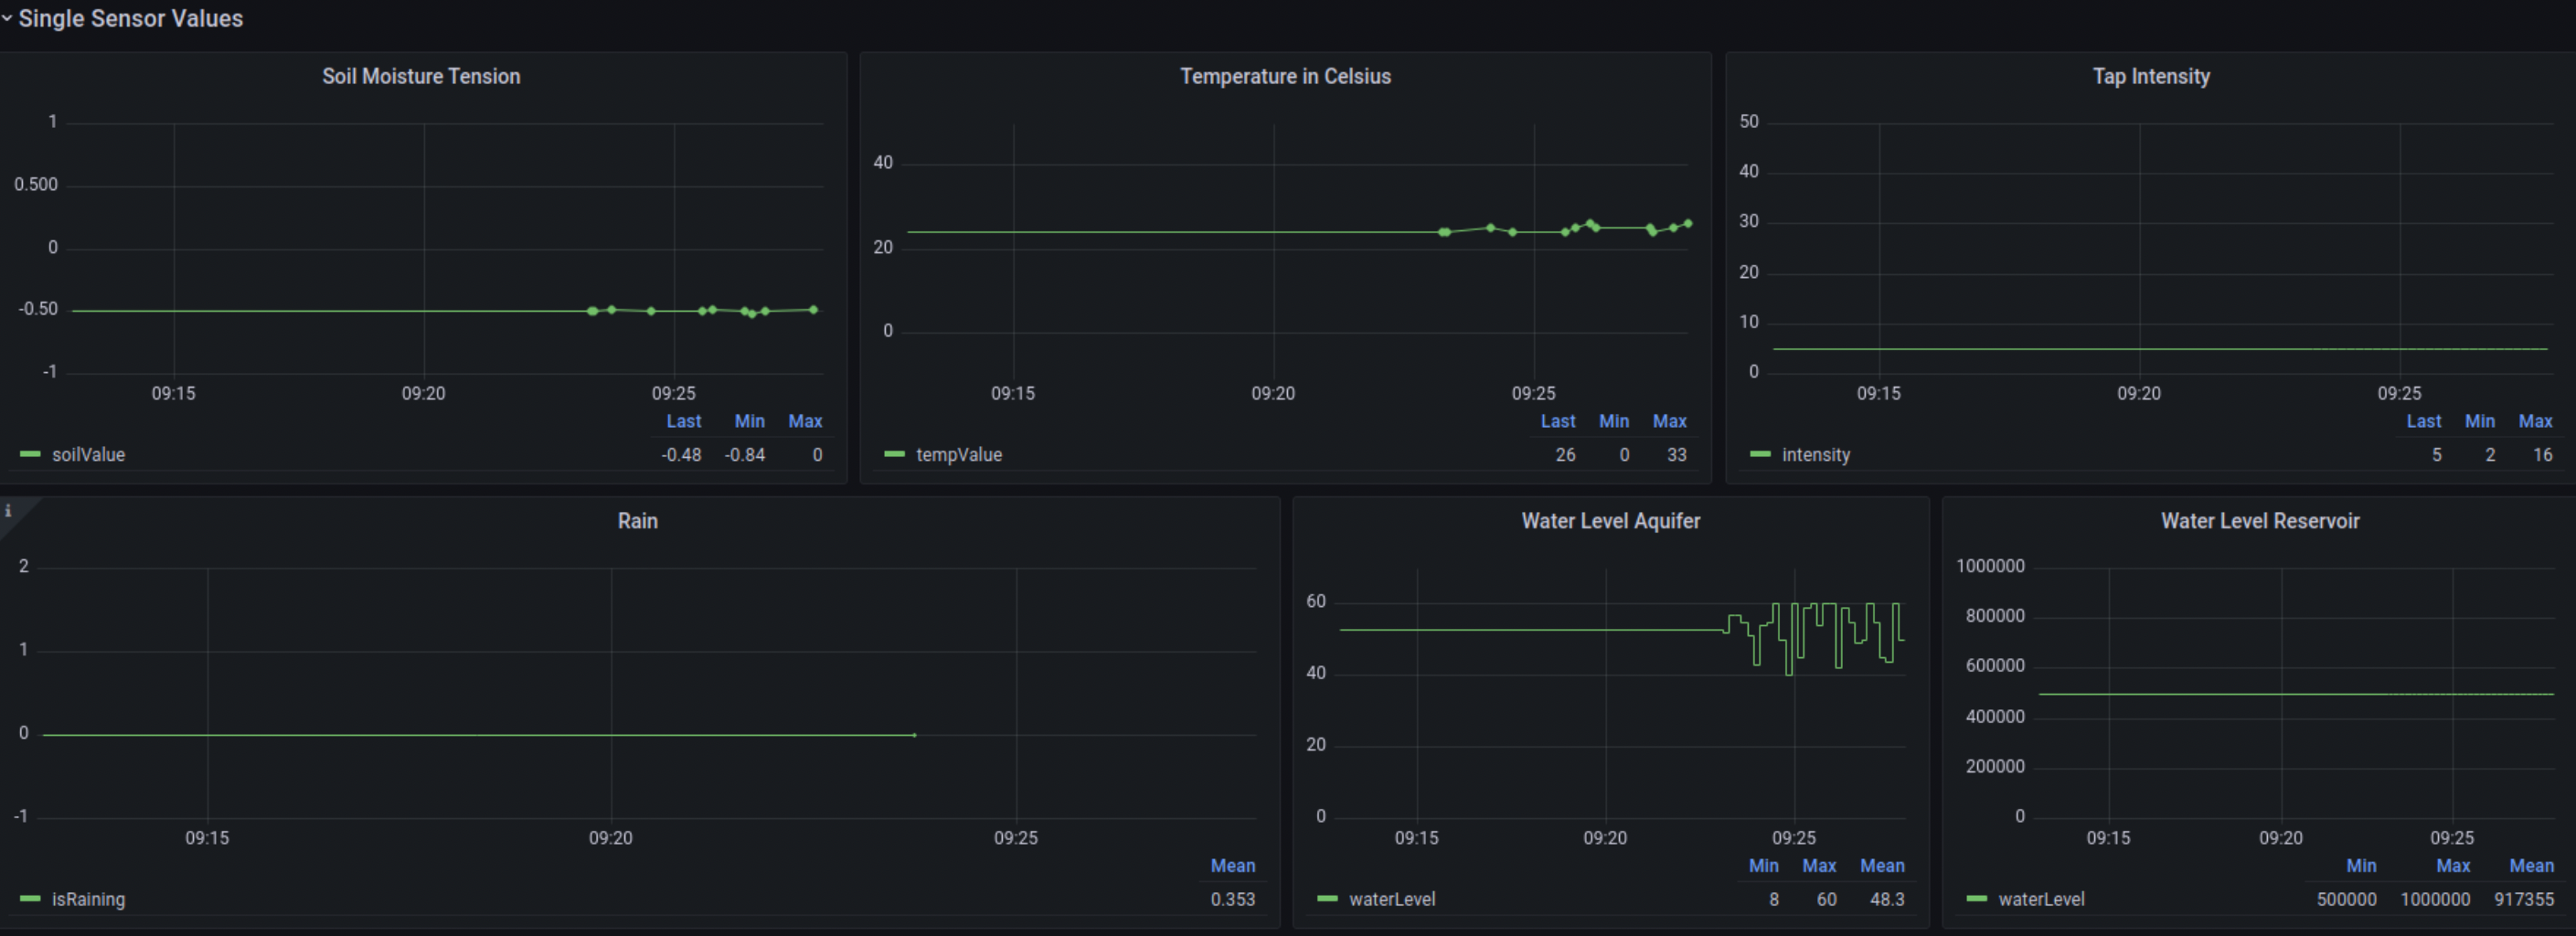
\includegraphics[width=1\linewidth]{img/grafana.png} 
	\end{subfigure}
\end{figure}

\subsection{Automatic Irrigation System}
The Automatic Irrigation System is the hearth of the proposed solution: it is in charge of periodically computing the water need based on data reported by the CoAP sensors and selecting the water source based on the measurements of the MQTT devices. The Automatic Irrigation System is a parallel Java Thread that can be started or stopped at any time by the user. At every iteration the system:
\begin{itemize}
	\item Collects into a Parameters object all the retrieved data needed to estimate the water need
	\item Computes the need based on the following formula: 

\begin{lstlisting}
if(p.isRaining){
  Logger.log("[Irrigation System]: It's Raining, no irrigation is needed");
  continue;
}

switch(p.soilStatus){
   case TOO_LOW:
       level = Levels.HIGH;
       break;
   case NORMAL:
       level = Levels.MEDIUM;
       break;
   default:
       level = Levels.LOW;
}
if (p.temperatureStatus == BoundStatus.TOO_HIGH)
     level = level.increaseLevel();

\end{lstlisting}


	\item Determines the actual tap output, given by \textit{level*tapIntensity}.
	\item Determines the water source, based on the water policy reported in the first paragraph and implemented as follows.

\begin{lstlisting}
if (need>p.aquiferLevel)
    WhereWater=RESERVOIR;
WhereWater=AQUIFER;
\end{lstlisting}	
	
	\item Sends a command to the reservoir to fetch/store water
\begin{lstlisting}
if (source == RESERVOIR){
     rc.changeReservoirLevel(0-quantity);
     Logger.log("\tFetched "+quantity + " from the RESERVOIR");
}
else{
     rc.changeReservoirLevel(p.aquiferLevel-quantity);
     Logger.log("\tFetched "+p.aquiferLevel+"cm^3 from the aquifer");
     Logger.log("\t" + quantity + "cm^3 of them are output of the tap,");
     Logger.log("\t" + (p.aquiferLevel-quantity) + "cm^3 of them are stored in the reservoir");
}
\end{lstlisting}
\end{itemize}



\end{document}